\section{Additional Experimental Results}


In this section, we provide comprehensive experimental results through our extensive neural architectural search. 



\subsection{All Neural Models} \label{app:a1}

All NXRO models share a common structure: they learn a vector field $f_\theta(X, t)$ that defines an ordinary differential align* (ODE) for the state evolution:
\begin{align*}
    \frac{dX}{dt} = f_\theta(X, t)
\end{align*}
where $X \in \mathbb{R}^d$ is the state vector containing climate indices (e.g., Ni\~no3.4, WWV, NPMM, etc.), $t$ is time in years, and $\theta$ represents learnable parameters. All models use a Fourier time embedding to capture seasonality:
\begin{align*}
    \phi(t) = \left[1, \cos(\omega t), \sin(\omega t), \ldots, \cos(K\omega t), \sin(K\omega t)\right]^\top \in \mathbb{R}^{1+2K}
\end{align*}
with $\omega = 2\pi$ (annual cycle) and $K=2$ (default) giving 5 basis functions.

\textbf{Default Hyperparameters:} Epochs: 2000, batch size: 128, learning rate: $10^{-3}$, weight decay: $10^{-4}$, $K=2$.

%==============================================================================
\paragraph{NXRO-Linear.}
A purely linear model with seasonally-varying linear operator.
\begin{align*}
    \frac{dX}{dt} = L_\theta(t) \cdot X, \quad L_\theta(t) = \sum_{k=0}^{2K} W_k \cdot \phi_k(t)
\end{align*}
where $W_k \in \mathbb{R}^{d \times d}$ are learnable weight matrices. \textbf{Params:} $5d^2$.

\begin{tabular}{@{}ll@{}}
\textbf{Variant} & \textbf{Description} \\
\hline
NXRO-Linear & Random Xavier initialization \\
NXRO-Linear-WS & Warm-start from XRO linear operator \\
\end{tabular}

%==============================================================================
\paragraph{NXRO-RO.}
Seasonal linear operator plus Recharge Oscillator (RO) nonlinear terms on $(T, H)$.
\begin{align*}
    \frac{dX}{dt} = L_\theta(t) \cdot X + \begin{bmatrix} \text{RO}_T(T,H,t) \\ \text{RO}_H(T,H,t) \\ 0 \\ \vdots \end{bmatrix}, \quad
    \text{RO}_T = \sum_{k} c^T_k(t) \cdot \psi_k(T,H)
\end{align*}
with $\psi = [T^2, TH, T^3, T^2H, TH^2]^\top$ and seasonally-varying coefficients.

%==============================================================================
\paragraph{NXRO-RO+Diag.}
Extends NXRO-RO with diagonal quadratic and cubic terms for all variables.
\begin{align*}
    \frac{dX}{dt} = L_\theta(t) \cdot X + \text{RO}(T,H,t) + b(t) \odot X^2 + c(t) \odot X^3
\end{align*}

\begin{tabular}{@{}ll@{}}
\textbf{Variant} & \textbf{Description} \\
\hline
NXRO-RO+Diag & Random initialization \\
NXRO-RO+Diag-WS & Warm-start all, train all \\
NXRO-RO+Diag-FixL & Freeze linear, train RO+Diag \\
NXRO-RO+Diag-FixRO & Freeze RO, train linear+Diag \\
NXRO-RO+Diag-FixDiag & Freeze diagonal, train linear+RO \\
NXRO-RO+Diag-FixNL & Freeze RO+Diag, train linear only \\
\end{tabular}

%==============================================================================
\paragraph{NXRO-MLP.}
Seasonal linear operator plus a residual 2-layer MLP.
\begin{align*}
    \frac{dX}{dt} = L_\theta(t) \cdot X + R_\theta([X, \phi(t)]), \quad
    R_\theta(z) = W_3 \tanh(W_2 \tanh(W_1 z))
\end{align*}
\textbf{Hyperparams:} Hidden: 64, 2 layers, $\tanh$ activation.

\begin{tabular}{@{}ll@{}}
\textbf{Variant} & \textbf{Description} \\
\hline
NXRO-MLP & Random initialization \\
NXRO-MLP-WS-FixL & Warm-start \& freeze linear, train MLP only \\
\end{tabular}

%==============================================================================
\paragraph{NXRO-DeepMLP.}
General neural ODE with configurable-depth drift MLP and optional structural constraints.
\begin{align*}
    \frac{dX}{dt} = L_\theta(t) \cdot X + G_\theta([X, \phi(t)]) + M \cdot X
\end{align*}
where $G_\theta$ is a deeper MLP and $M$ is an optional masked linear mixing term.

%==============================================================================
\paragraph{NXRO-PhysReg.}
Neural ODE with physics-informed regularization via Jacobian penalty.
\begin{align*}
    \mathcal{L} = \mathcal{L}_{\text{MSE}} + \lambda_{\text{jac}} \|\nabla_X f_\theta(X,t)\|_F^2
\end{align*}
\textbf{Hyperparams:} Same as NXRO-DeepMLP, $\lambda_{\text{jac}} = 10^{-4}$.

%==============================================================================
\paragraph{NXRO-HybridMLP.}
Combines the interpretable RO+Diag structure with a scaled residual MLP.
\begin{align*}
    \frac{dX}{dt} = f_{\text{RO+Diag}}(X,t) + \alpha \cdot R_\theta([X, \phi(t)])
\end{align*}
\textbf{Hyperparams:} Hidden: 64, $\alpha_{\text{init}} = 0.1$, $\alpha_{\max} = 0.5$.

\begin{tabular}{@{}ll@{}}
\textbf{Variant} & \textbf{Description} \\
\hline
NXRO-HybridMLP & Random initialization \\
NXRO-HybridMLP-WS & Warm-start physics, train all \\
NXRO-HybridMLP-FixPhysics & Freeze RO+Diag, train MLP only \\
NXRO-HybridMLP-FixRO & Freeze RO terms only \\
NXRO-HybridMLP-FixNL & Freeze all nonlinear physics \\
\end{tabular}

%==============================================================================
\paragraph{NXRO-Bilinear.}
Seasonal linear plus low-rank bilinear channels with seasonal gating.
\begin{align*}
    \frac{dX}{dt} = L_\theta(t) \cdot X + \sum_{c=1}^{C} \alpha_c(t) \cdot s_c(X) \cdot W^{(c)}_{\text{proj}}
\end{align*}
where $s_c(X) = \sum_r (P_c^\top X)_r (Q_c^\top X)_r$ are bilinear scalars. \textbf{Hyperparams:} Channels: 2, rank: 2.

%==============================================================================
\paragraph{NXRO-Attention.}
Seasonal linear plus lightweight self-attention across variables.
\begin{align*}
    \frac{dX}{dt} = L_\theta(t) \cdot X + \alpha(t) \cdot \text{Proj}\left(\text{softmax}\left(\frac{M \odot QK^\top}{\sqrt{d_k}}\right) V\right)
\end{align*}
\textbf{Hyperparams:} $d=32$, single head. \textbf{Mask:} \texttt{th\_only} (attend from $T,H$) or \texttt{full}.

\begin{tabular}{@{}ll@{}}
\textbf{Variant} & \textbf{Description} \\
\hline
NXRO-Attention & Random initialization \\
NXRO-Attention-WS & Warm-start linear, train all \\
NXRO-Attention-FixL & Freeze linear, train attention only \\
\end{tabular}

%==============================================================================
\paragraph{NXRO-Graph.}
Seasonal linear plus sparse graph-based drift.
\begin{align*}
    \frac{dX}{dt} = L_\theta(t) \cdot X + \alpha(t) \cdot \tanh\left(\hat{A} X \cdot W_g\right)
\end{align*}
where $\hat{A}$ is a row-normalized adjacency matrix. \textbf{Hyperparams:} Top-$k$: 2.

\begin{tabular}{@{}ll@{}}
\textbf{Variant} & \textbf{Description} \\
\hline
NXRO-Graph-Fixed & Fixed adjacency from XRO or correlation \\
NXRO-Graph-Learned & Learnable adjacency with L1 reg ($\lambda_1 = 0.01$) \\
\end{tabular}

%==============================================================================
\paragraph{NXRO-GCN.}
PyTorch Geometric-based Graph ODE using Graph Convolutional Networks. This is the NXRO-GNN model in the main paper.

\begin{align*}
    \frac{dX}{dt} = L_\theta(t) \cdot X + \alpha(t) \cdot \text{GCN}_\theta(X, \mathcal{E})
\end{align*}
Two GCNConv layers with $\tanh$ activation. \textbf{Hyperparams:} Hidden: 16, top-$k$: 3, dropout: 0.1.

%==============================================================================
\paragraph{NXRO-GAT.}
PyTorch Geometric-based Graph ODE using Graph Attention Networks.
\begin{align*}
    \frac{dX}{dt} = L_\theta(t) \cdot X + \alpha(t) \cdot \text{GAT}_\theta(X, \mathcal{E})
\end{align*}
Same as NXRO-GCN but uses GATConv with attention-weighted message passing:
\begin{align*}
    h_i = \sigma\left(\sum_{j \in \mathcal{N}(i)} \alpha_{ij} W h_j\right), \quad \alpha_{ij} \propto \exp(\text{LeakyReLU}(a^\top [Wh_i \| Wh_j]))
\end{align*}
\textbf{Hyperparams:} Hidden: 16, top-$k$: 3, dropout: 0.1.

%==============================================================================
\paragraph{NXRO-Transformer.}
Pure Transformer architecture treating each variable as a token.
\begin{align*}
    \frac{dX}{dt} = \text{OutputProj}\left(\text{TransformerEncoder}\left(\text{InputProj}([X_i, \phi(t)]) + p_i\right)_{i=1}^d\right)
\end{align*}
where $p_i$ is a learnable positional embedding for variable $i$.
\textbf{Hyperparams:} $d_{\text{model}}$: 64, heads: 4, layers: 2, FFN dim: 256, dropout: 0.1, GELU.

The comprehensive results of all model ranking, trained only on the ORAS5 dataset, can be found in Figure \ref{fig:all_models_rmse_ranking}.

\begin{figure}
    \centering
    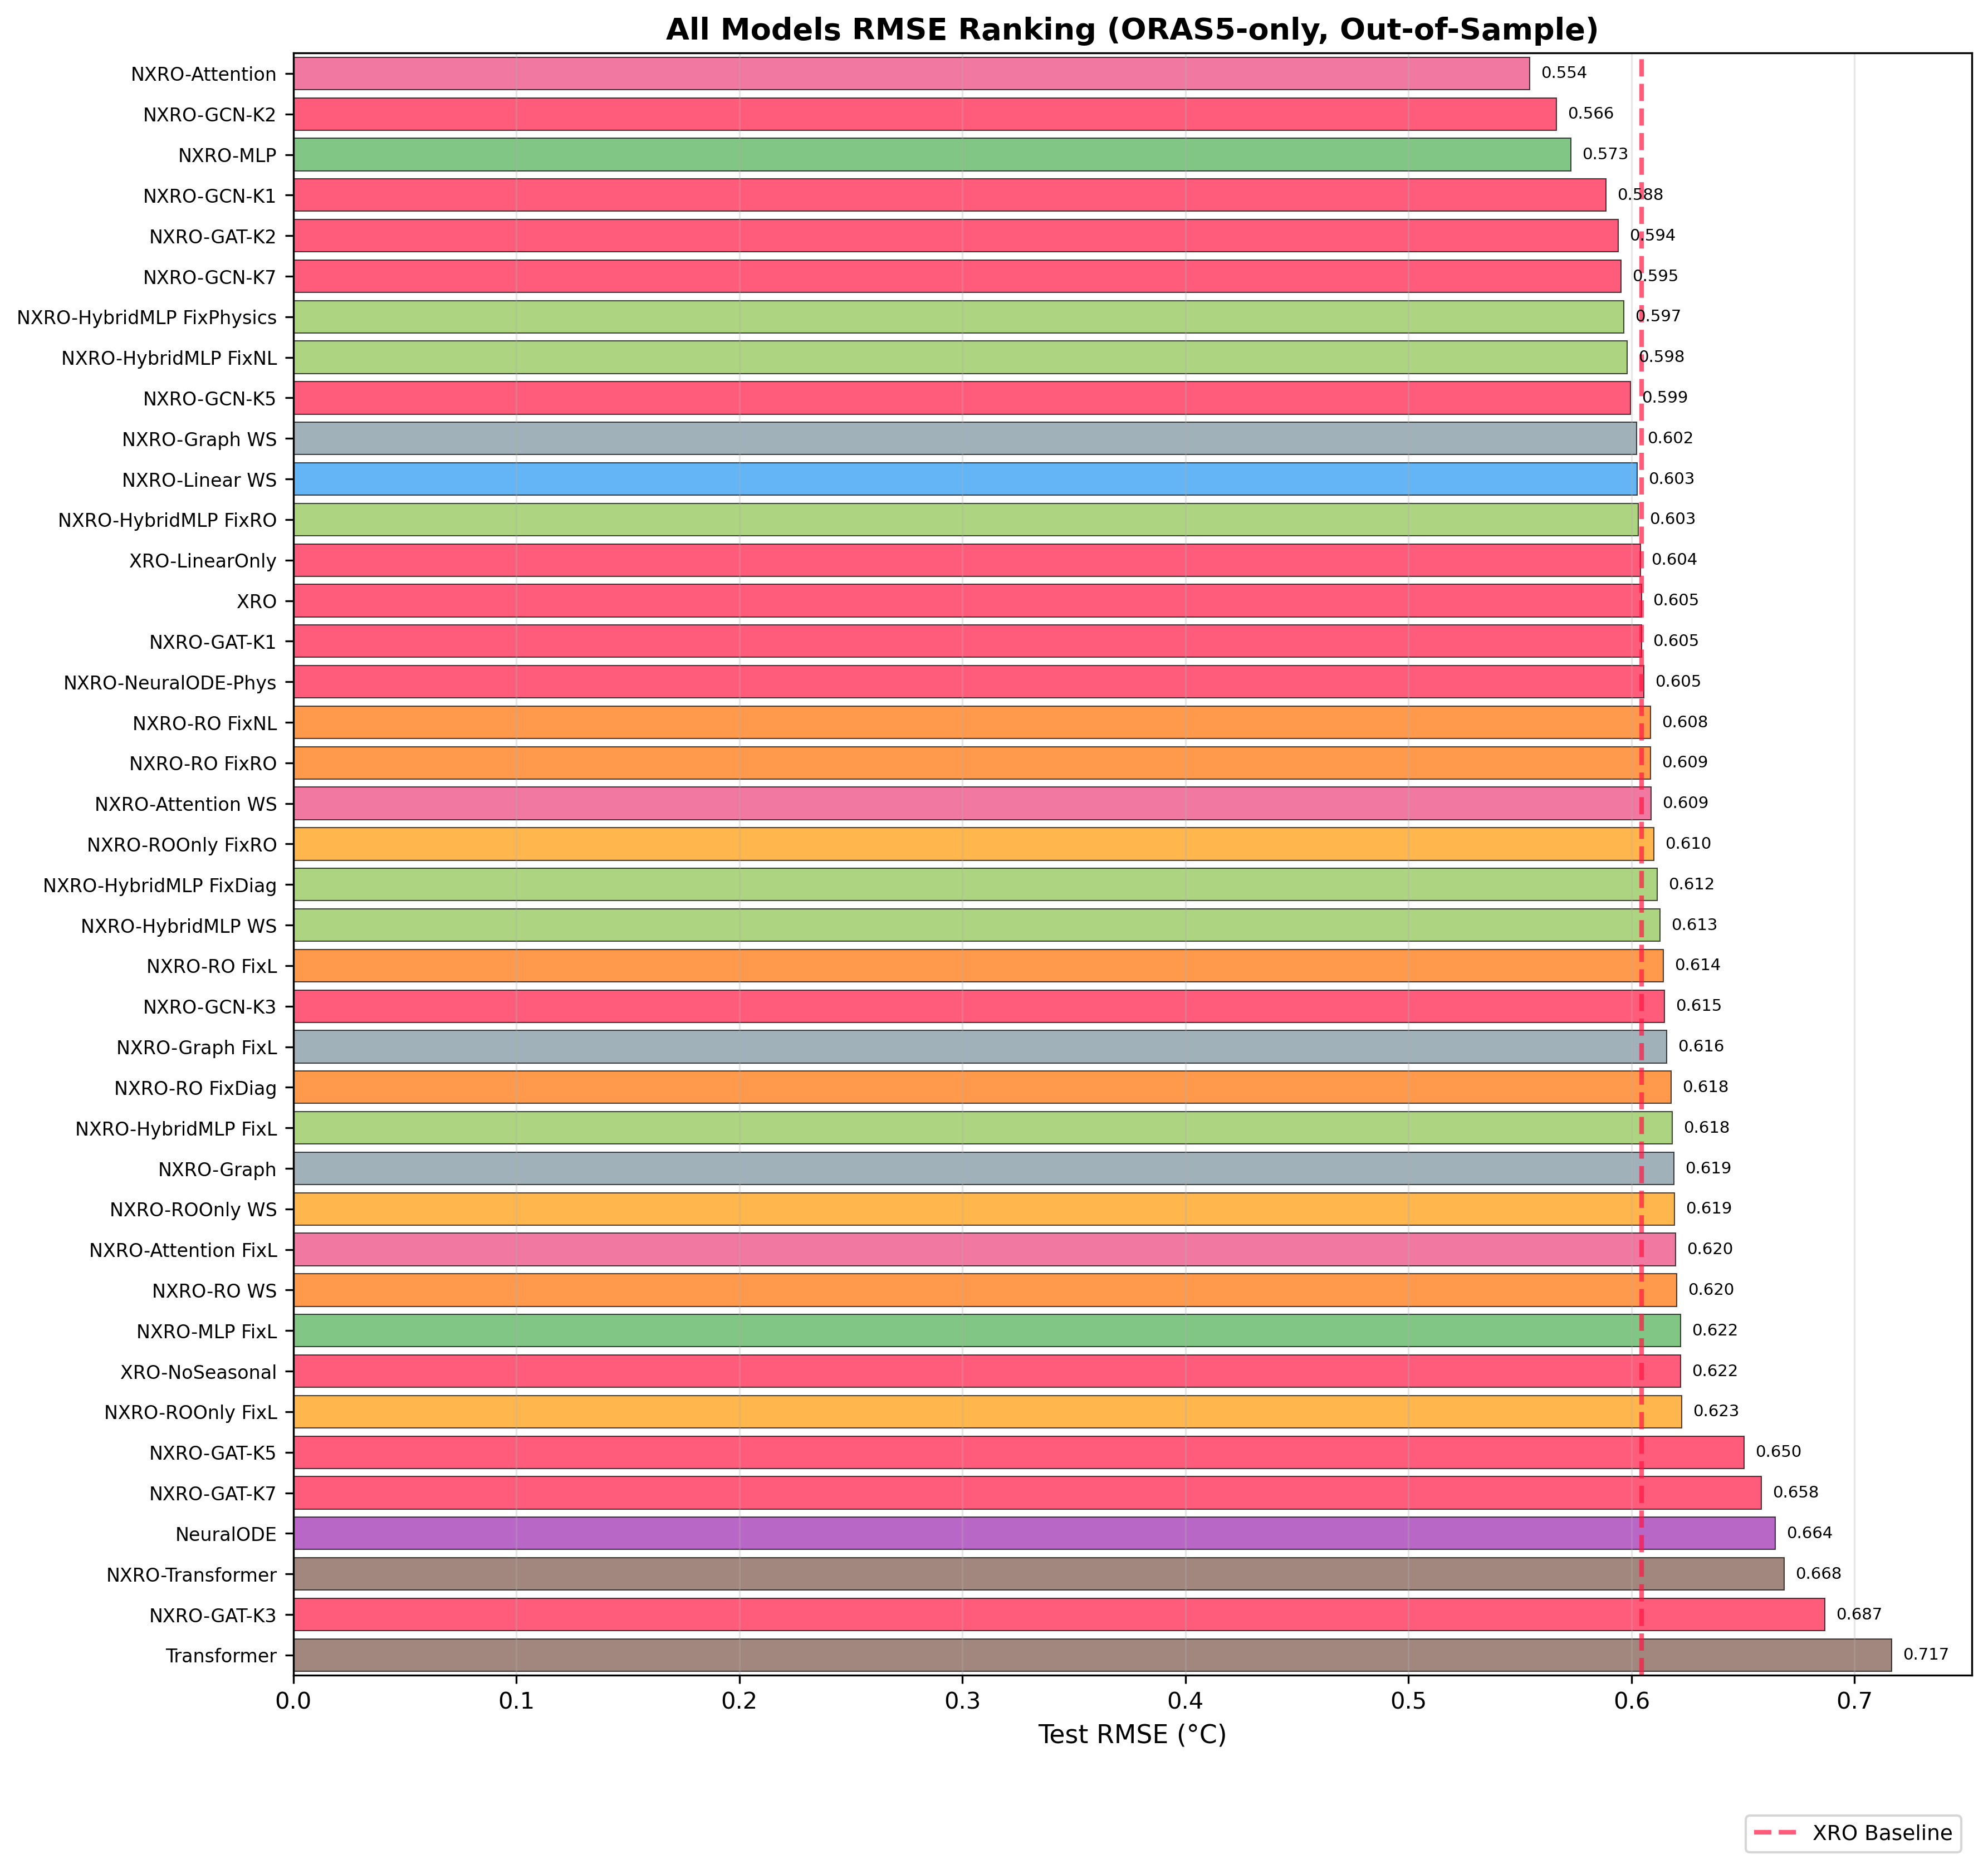
\includegraphics[width=0.9\linewidth]{figures/1_all_models_rmse_ranking.png}
    \caption{Comprehensive rankings for all models in the neural architecture search. About 18 models achieve better average RMSE results than the baseline model of XRO, with the best model to be the Neural XRO with MLP residual component.}
    \label{fig:all_models_rmse_ranking}
\end{figure}


\subsection{Complete End-to-End Results with Climate Simulation Data}

We present additional results for NXRO models trained using the CESM dataset pretraining + ORAS5 dataset finetuning set up. In this case, we only focus on the subset of NXRO models that do not use any warm-starts or parameter freezings, and fix the hyperparameter of NXRO variants that use graph neural network to only use the best hyperparameter found in the stage one setting. The results of the comprehensive RMSE result can be found in Figure \ref{fig:all_e2e_rmse_ranking}. The overall comprehensive ranking of all model variants (including both single stage training version and the end-to-end pretraining+finetuning version) can be found in Figure \ref{fig:all_rmse_ranking}, where the NXRO-MLP model still performs the best overall, despite its simplicity. 

\begin{figure}
    \centering
    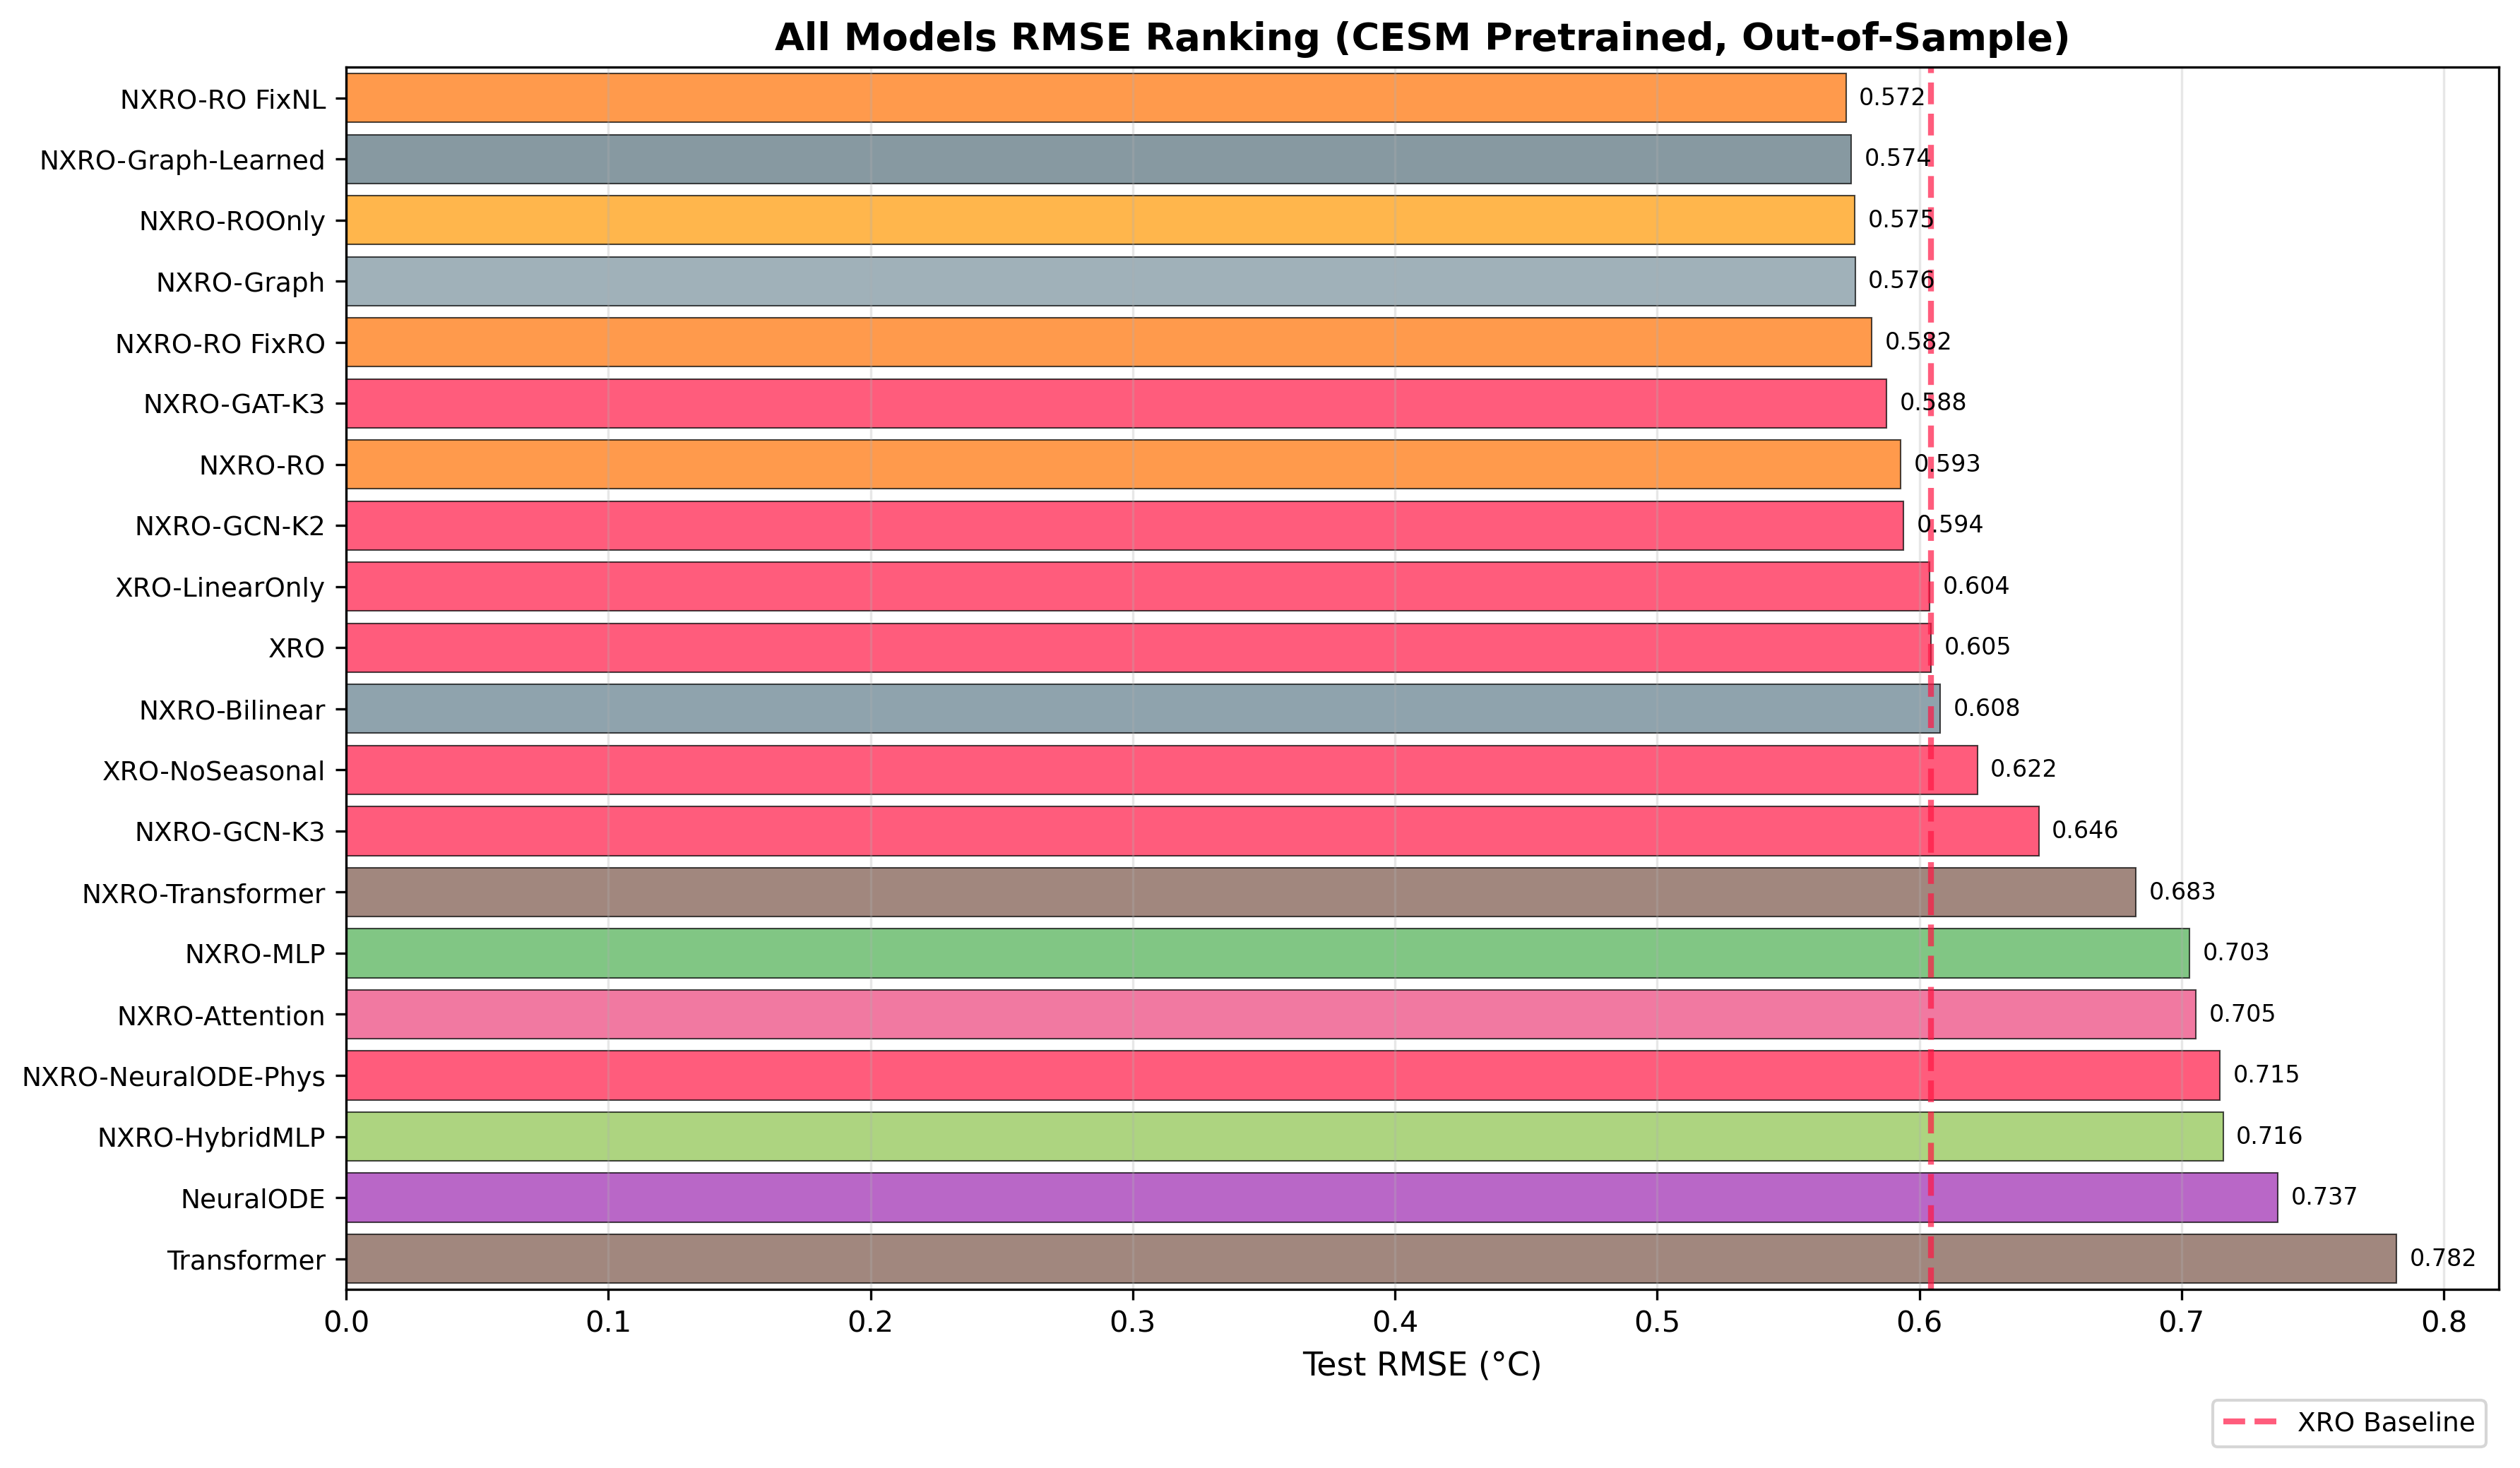
\includegraphics[width=\linewidth]{figures/2_all_models_rmse_ranking.png}
    \caption{The comprehensive results for all the selected NXRO variants, trained using the CESM-dataset training + ORAS5-dataset finetuning set up. It can be observed that the best performing models in the single-stage set up actually has degraded performance with the presence of more synthetic datasets, while many previously poor-performing models are improved.}
    \label{fig:all_e2e_rmse_ranking}
\end{figure}

\begin{figure}
    \centering
    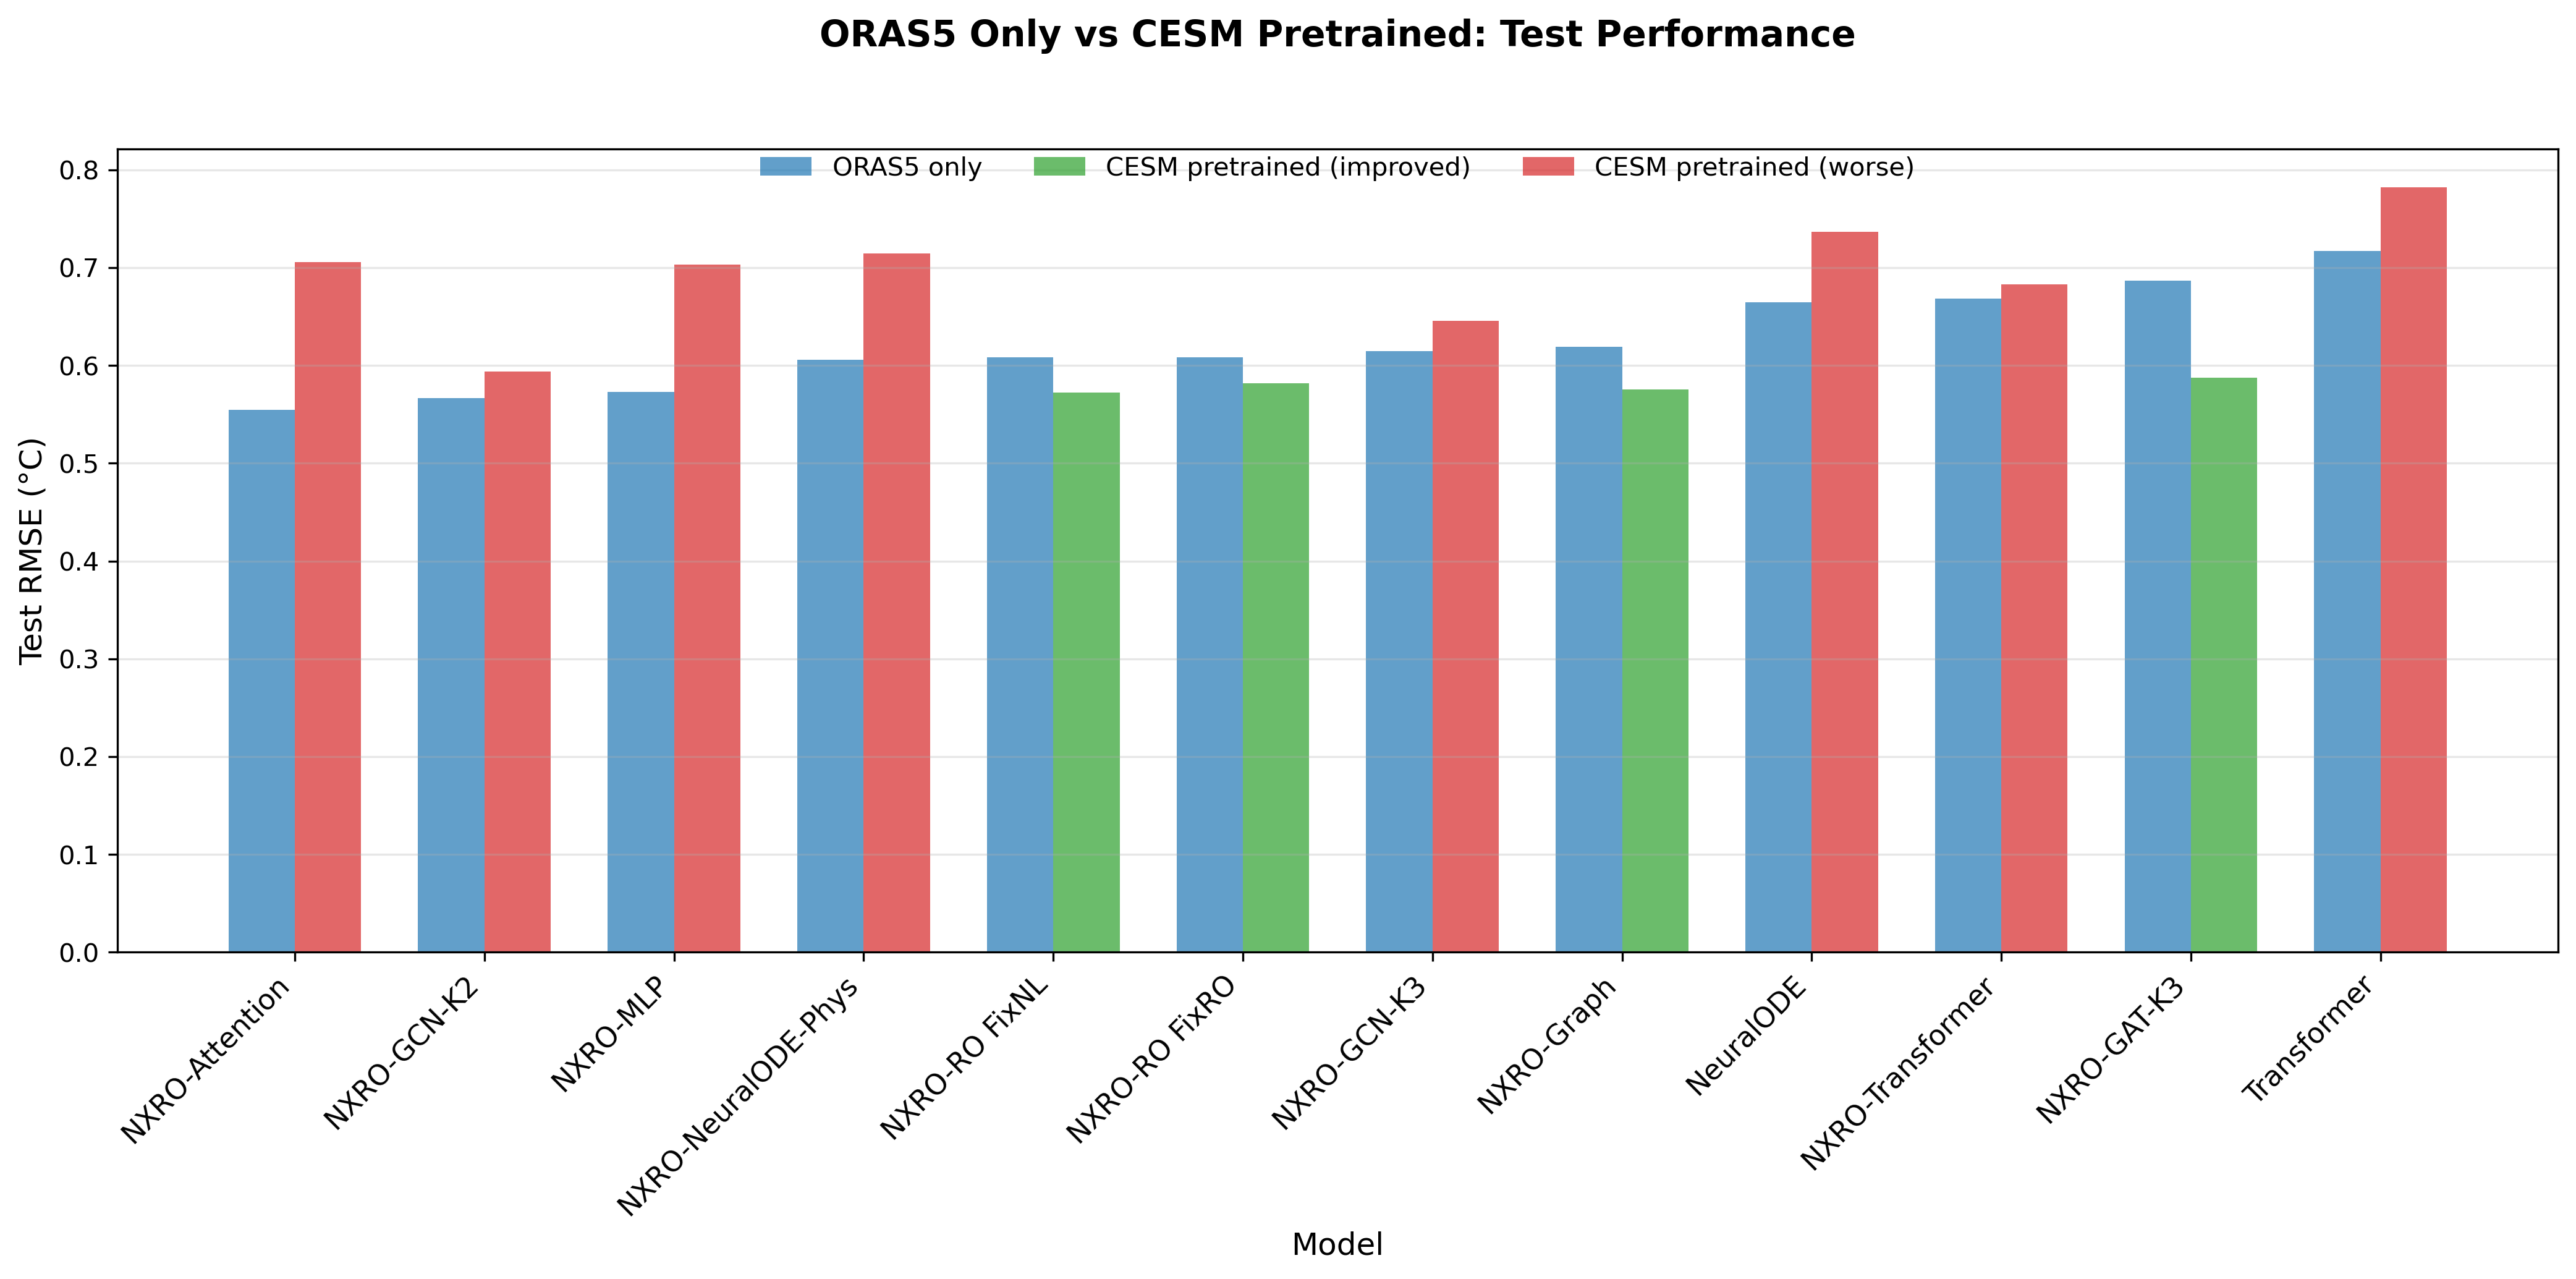
\includegraphics[width=\linewidth]{figures/6c_single_vs_two_stage_gap.png}
    \caption{Performance comparison of the same set of models with or without the pre-training step with the CESM climate simulation datasets.}
    \label{fig:one_vs_two}
\end{figure}

\begin{figure}
    \centering
    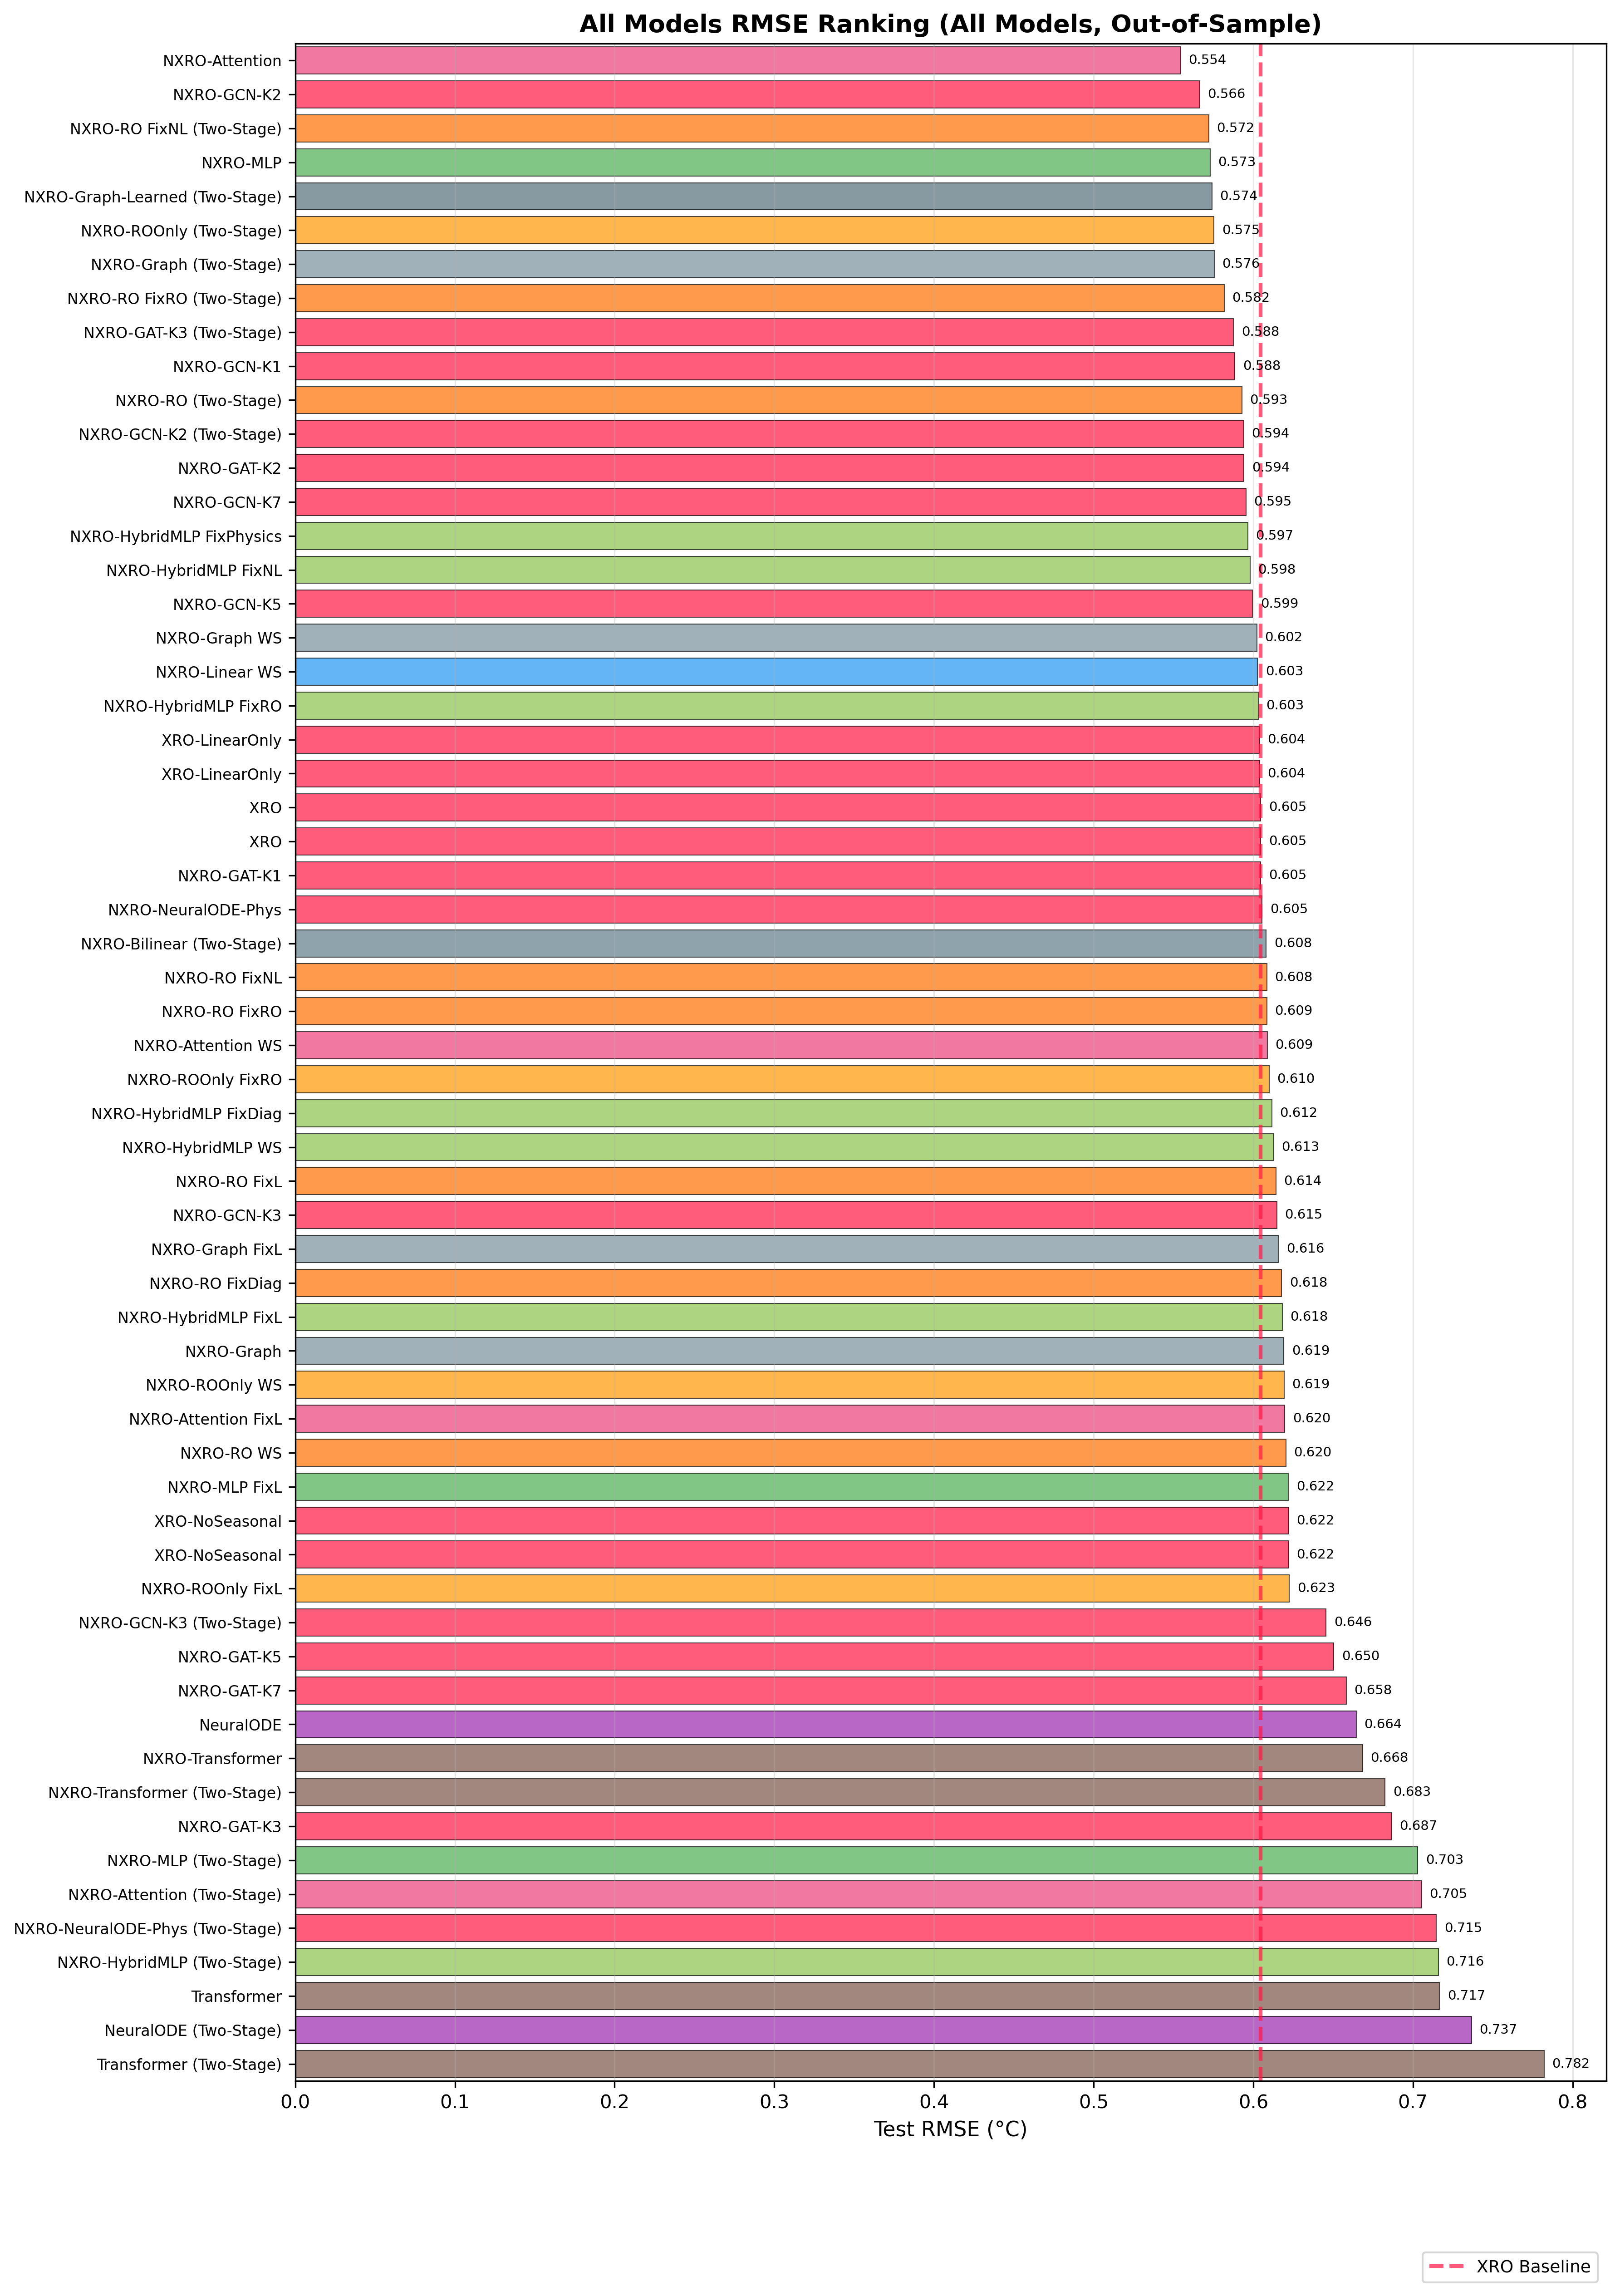
\includegraphics[width=0.9\linewidth]{figures/3_all_models_rmse_ranking.png}
    \caption{The overall ranking of all models, including both stage one-trained NXRO variants and NXRO variants trained using the CESM model simulation. Overall the NXRO-MLP model is still top-ranked.}
    \label{fig:all_rmse_ranking}
\end{figure}


The effect of pretraining on the CESM simulation dataset can be found in Figure \ref{fig:one_vs_two}. 



\subsection{ENSO Explainability with Graph Residual}

In this section, we present additional results by examining the learned KNN graph from the NXRO-Graph model. In the main paper, we have already presented the visualization of the learned adjacency matrix, the linear coupling strength between the climate indices, and the seasonal contribution from the nonlinear terms. Here we provide also \textbf{Seasonality Damping:} These are the diagonal elements $L_{ii}(t)$ of the coupling matrix across all 12 months. In this case, negative values indicate damped variable while positive values indicate amplification. The pattern shows that ENSO tends to be damped in Spring and peak in winter, which agrees with the observation. The results are in Figure \ref{fig:gcn_damping}. For completeness, we also show the statistics of the graph structure learned in the NXRO-GNN model in Figure \ref{fig:gcn_hubs}

\begin{figure}
    \centering
    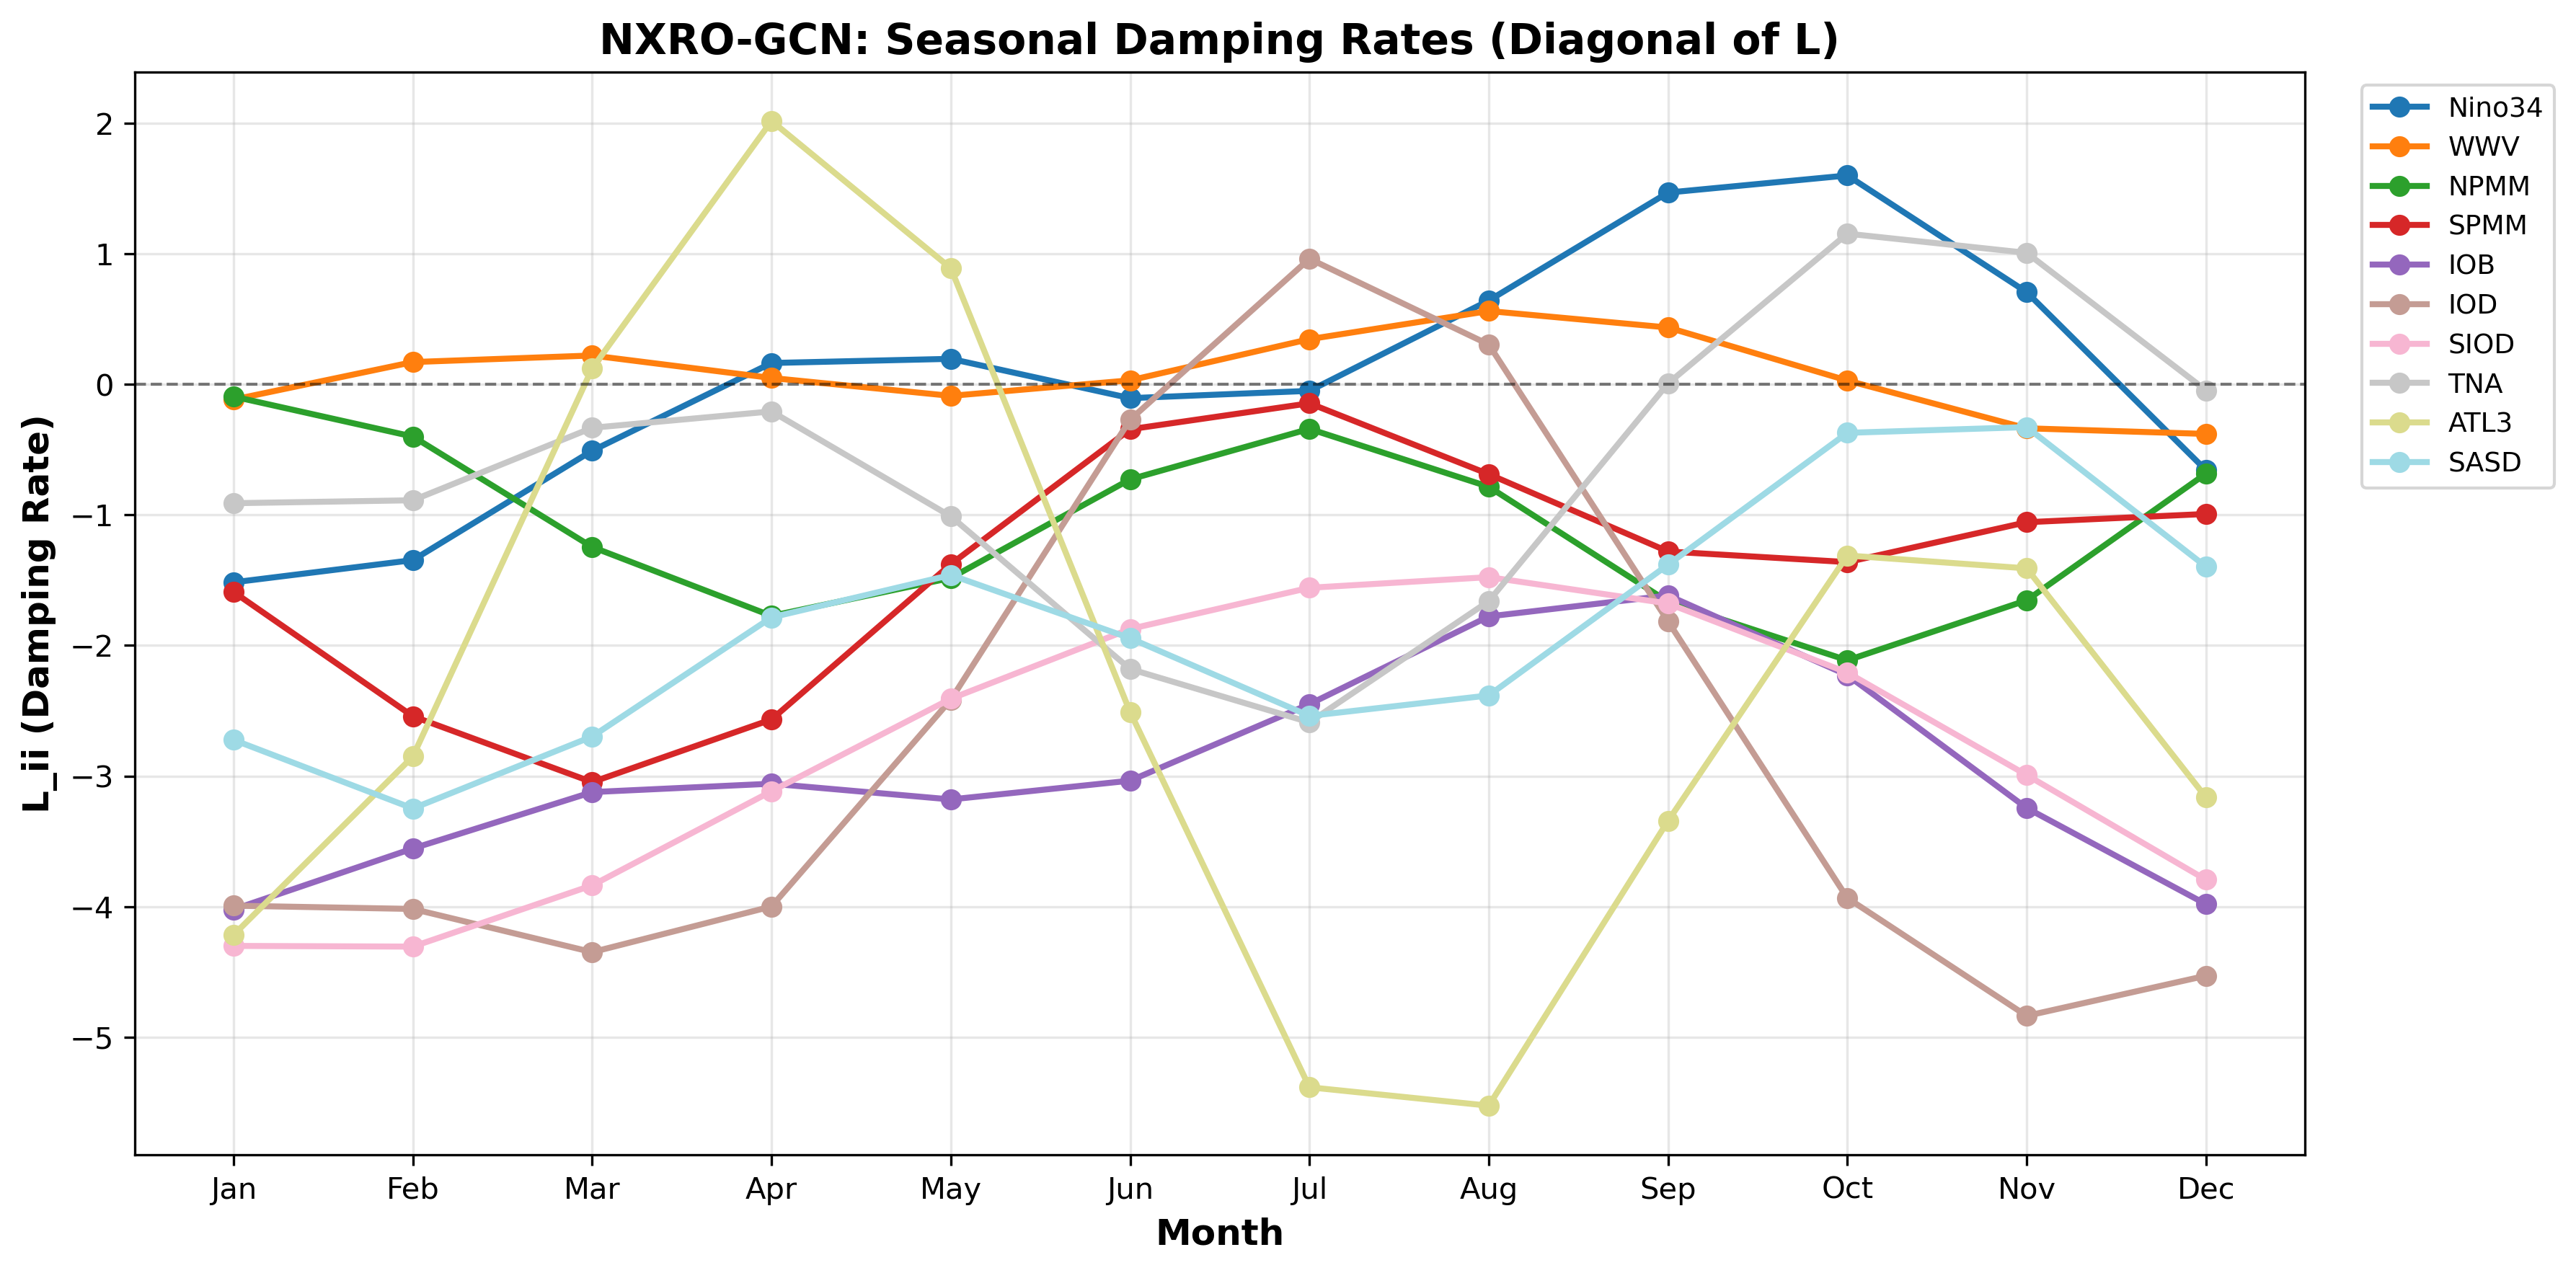
\includegraphics[width=\linewidth]{figures/gcn_damping_rates.png}
    \caption{Seasonality Damping coefficients of learned NXRO-GCN model. This shows the model learned damping factor for each index across different months.}
    \label{fig:gcn_damping}
\end{figure}


\begin{figure}
    \centering
    
\includegraphics[width=\linewidth]{sections/connections_and_hubs.png}
    \caption{The connection and hubs from the learned graph using the NXRO-GNN model with a learnable graph structure.}
    \label{fig:gcn_hubs}
\end{figure}




% \subsection{ENSO Explainability with Attention Residual}




% \begin{figure}
%     \centering
%     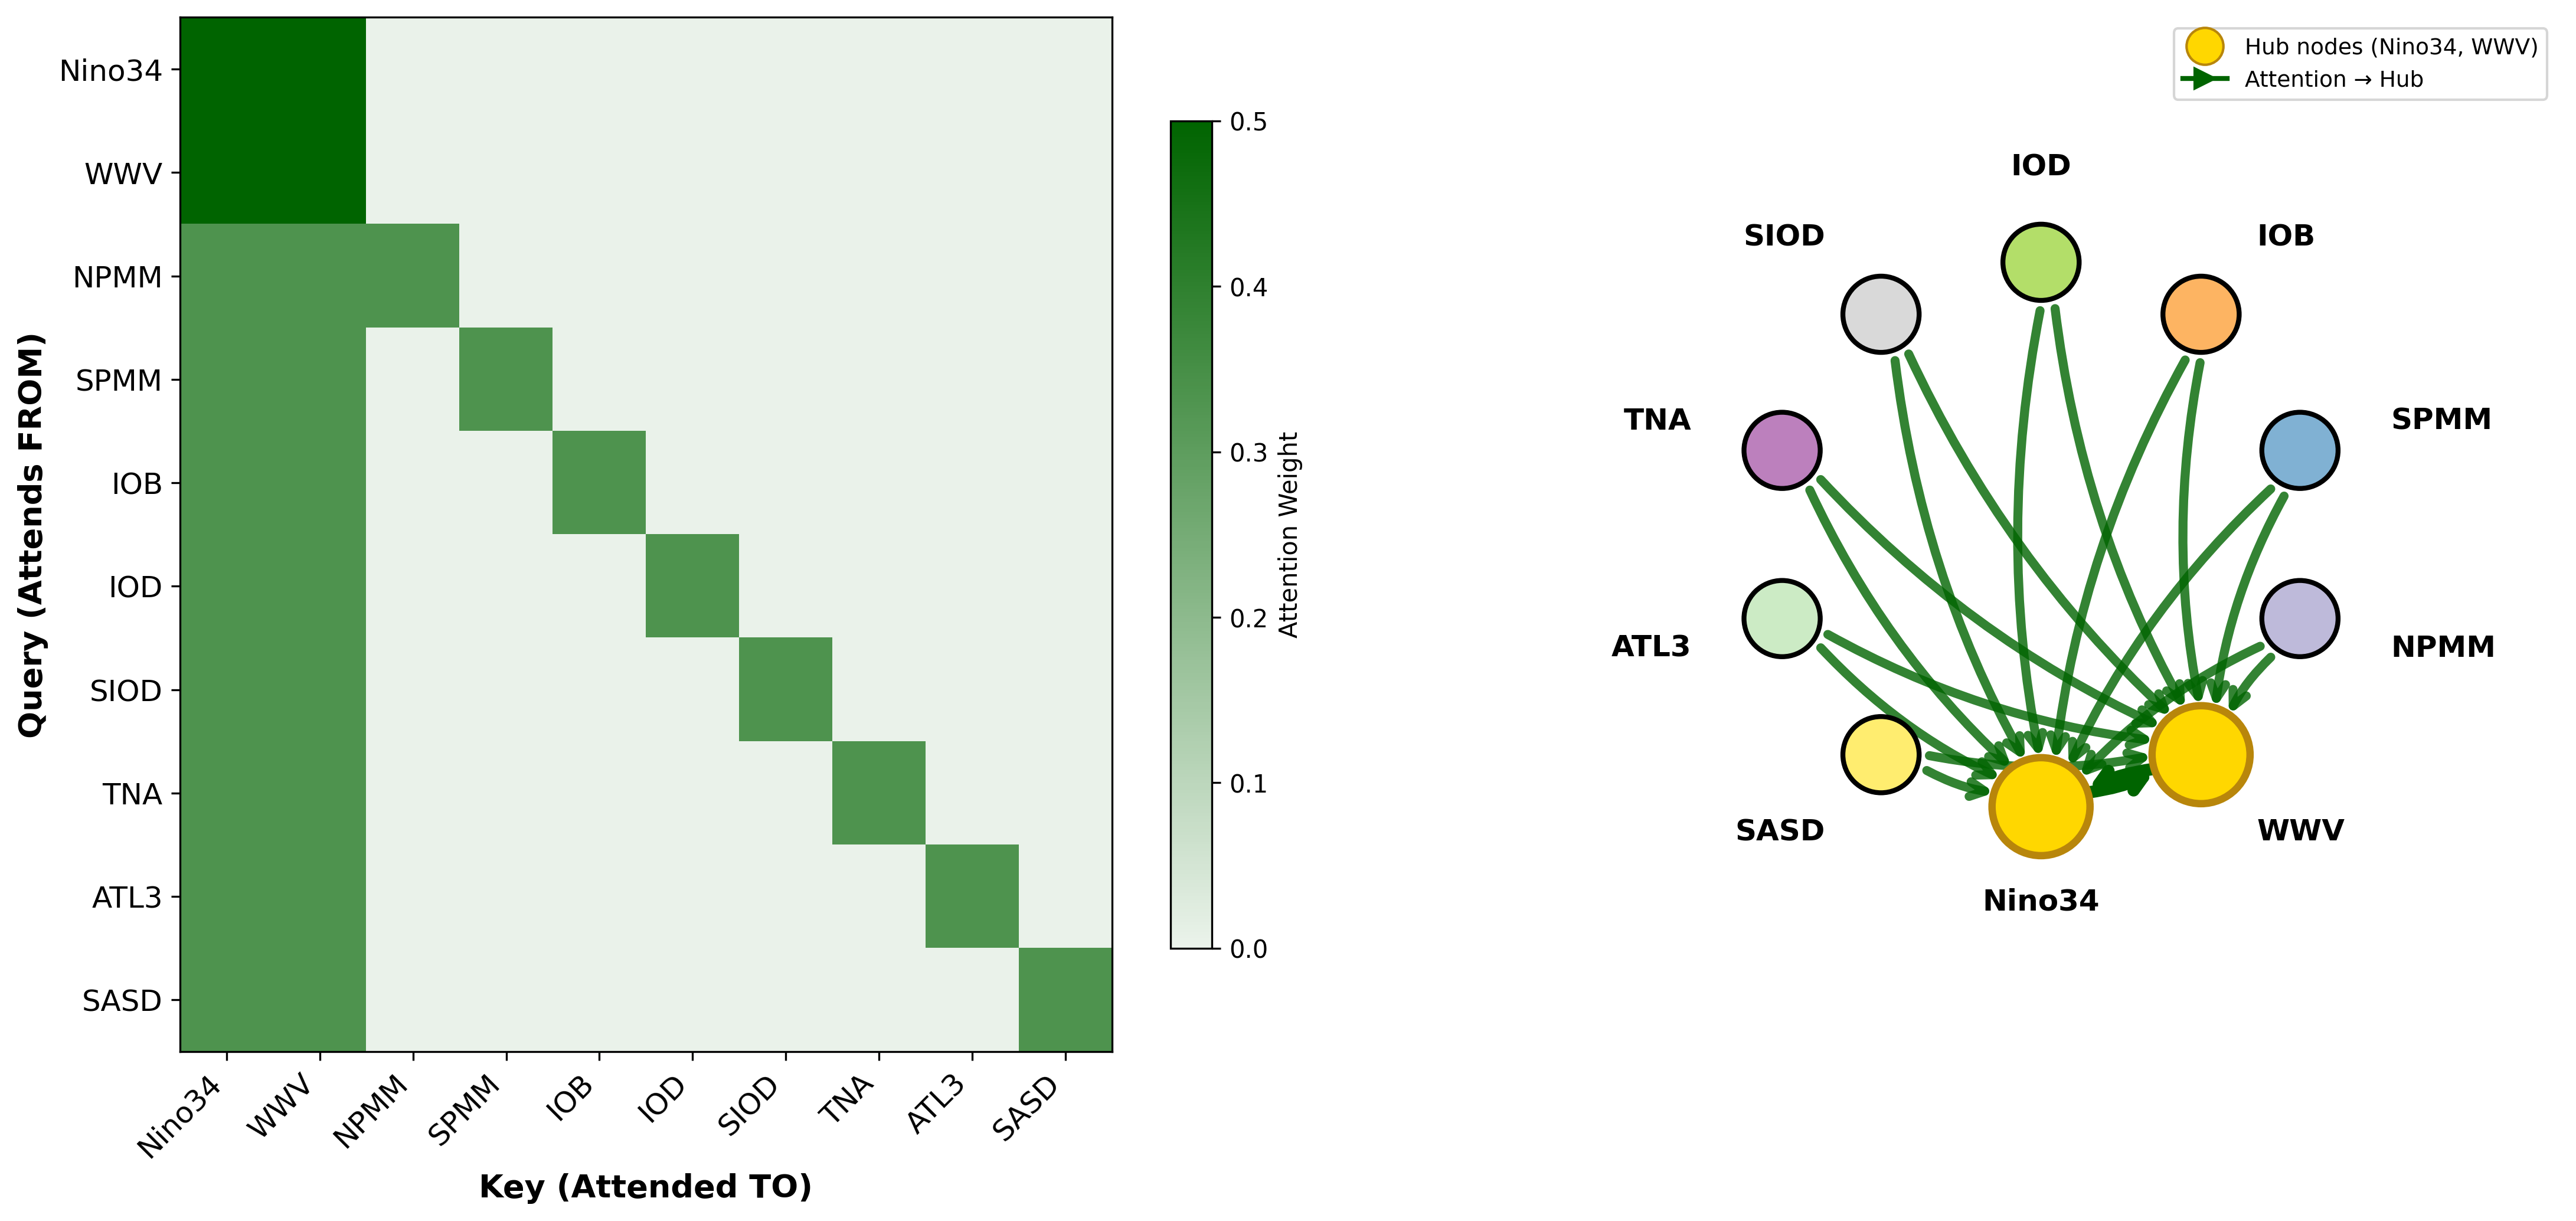
\includegraphics[width=\linewidth]{figures/attention_adjacency_and_network.png}
%     \caption{NXRO-Attention learned attention masking for interaction between components.}
%     \label{fig:attn_network}
% \end{figure}


% \begin{figure}
%     \centering
%     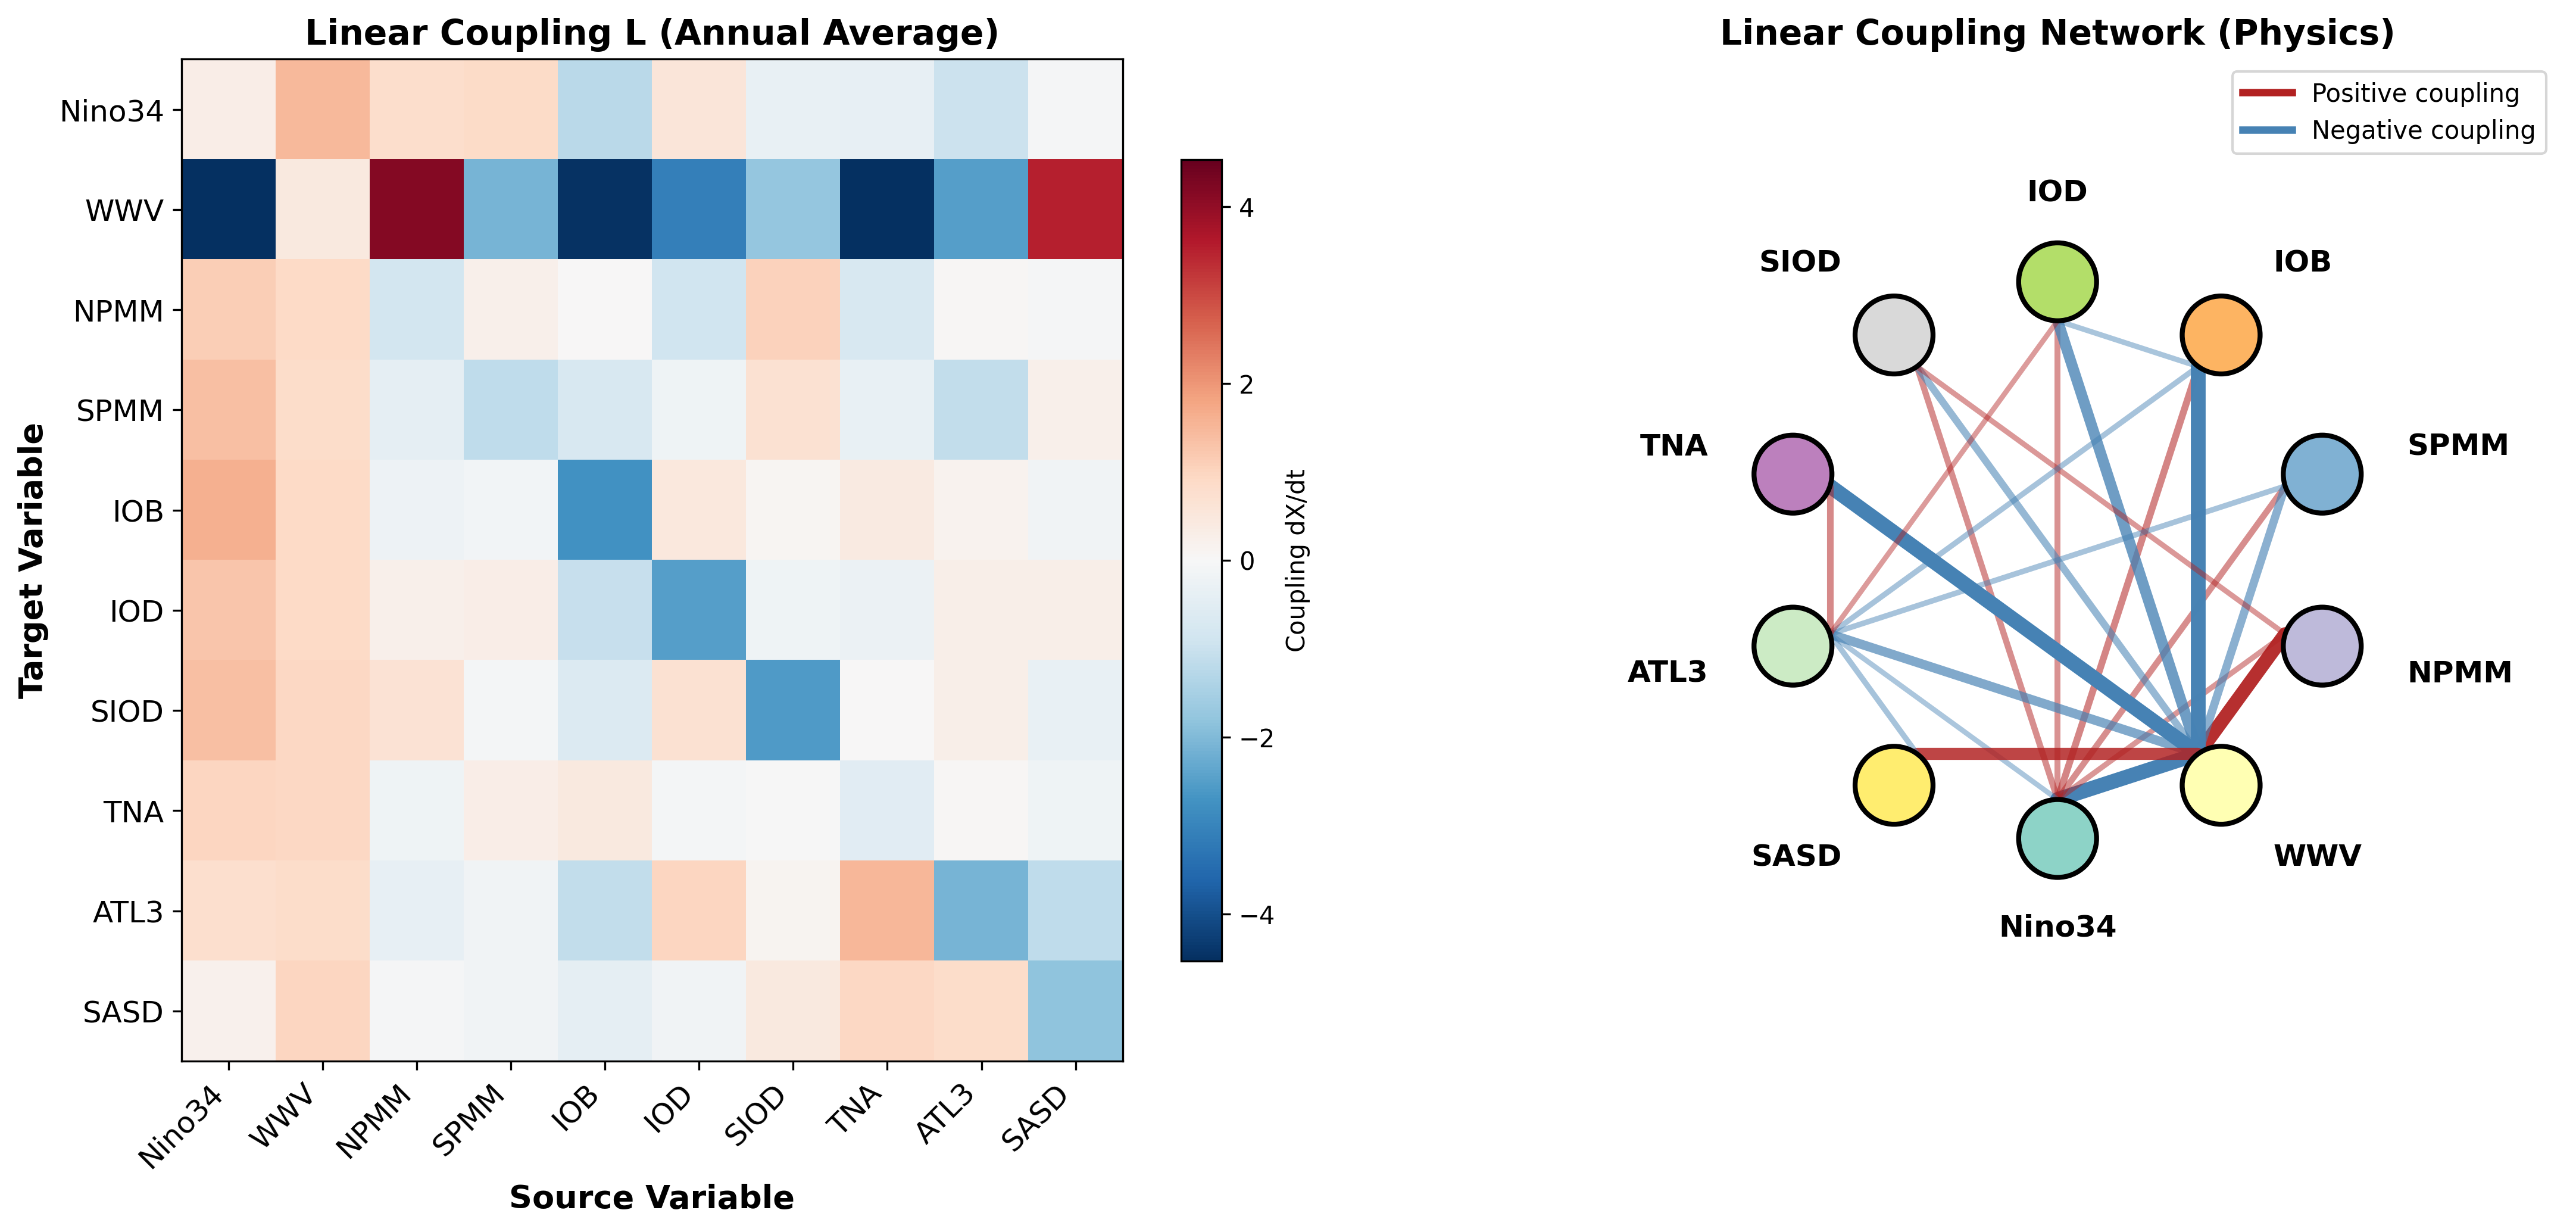
\includegraphics[width=\linewidth]{figures/attention_linear_coupling_L.png}
%     \caption{XNRO-Attention  model's learned linear component, demonstrating the strength of linear interaction strength between the climate modes.}
%     \label{fig:attn_linear}
% \end{figure}


% \begin{figure}
%     \centering
%     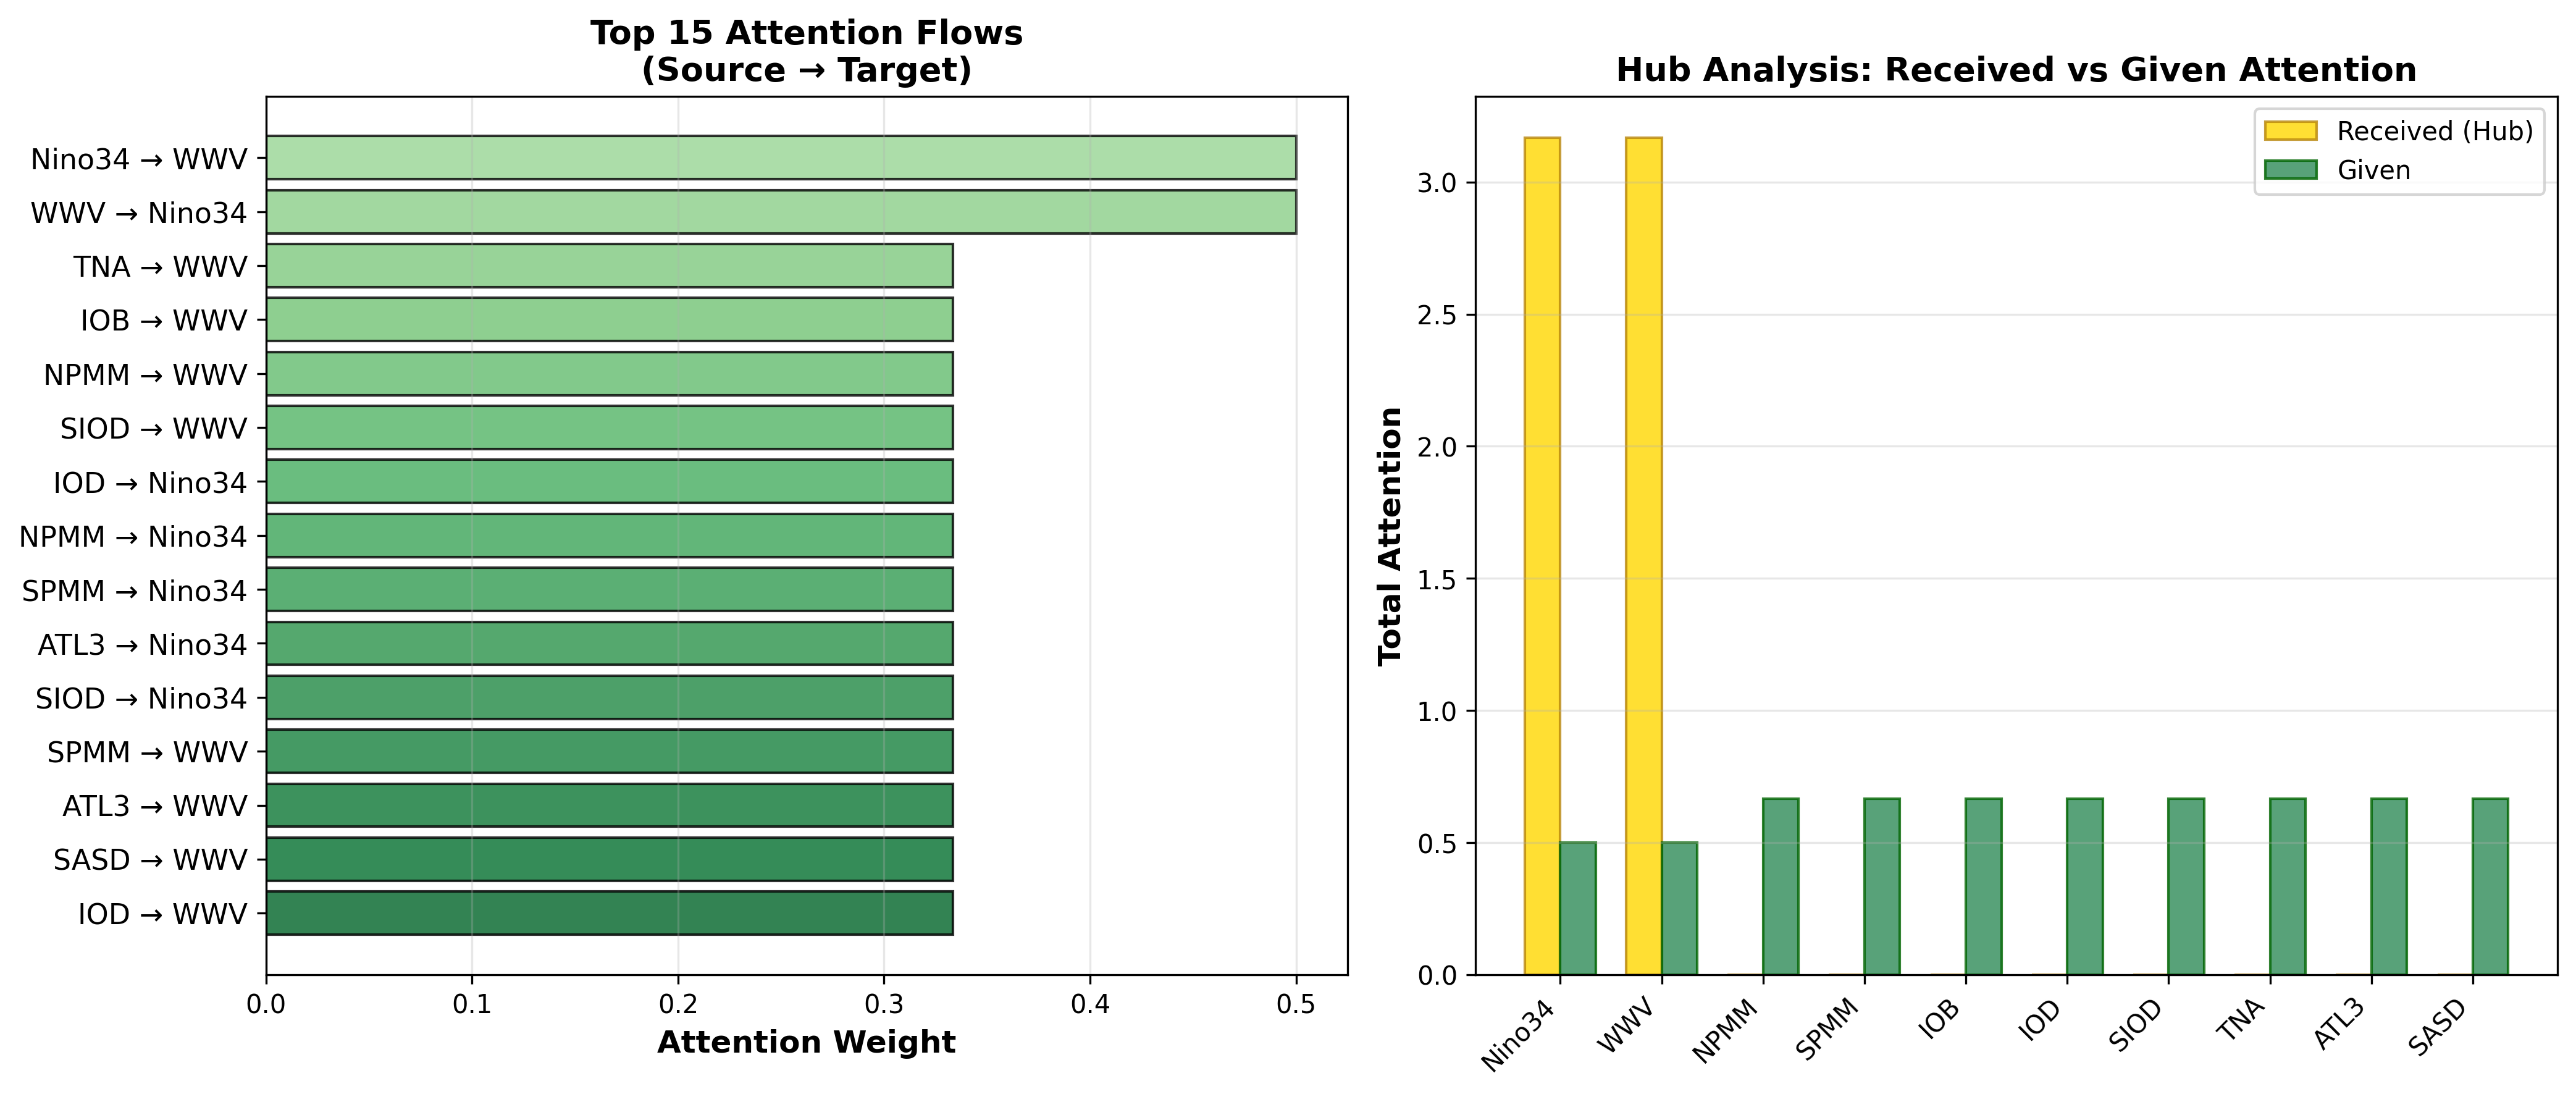
\includegraphics[width=\linewidth]{figures/attention_connections_and_hubs.png}
%     \caption{The connection and hubs from the learned NXRO-Attention model with learnable attention masking.}
%     \label{fig:attn_hubs}
% \end{figure}



% \begin{figure}
%     \centering
%     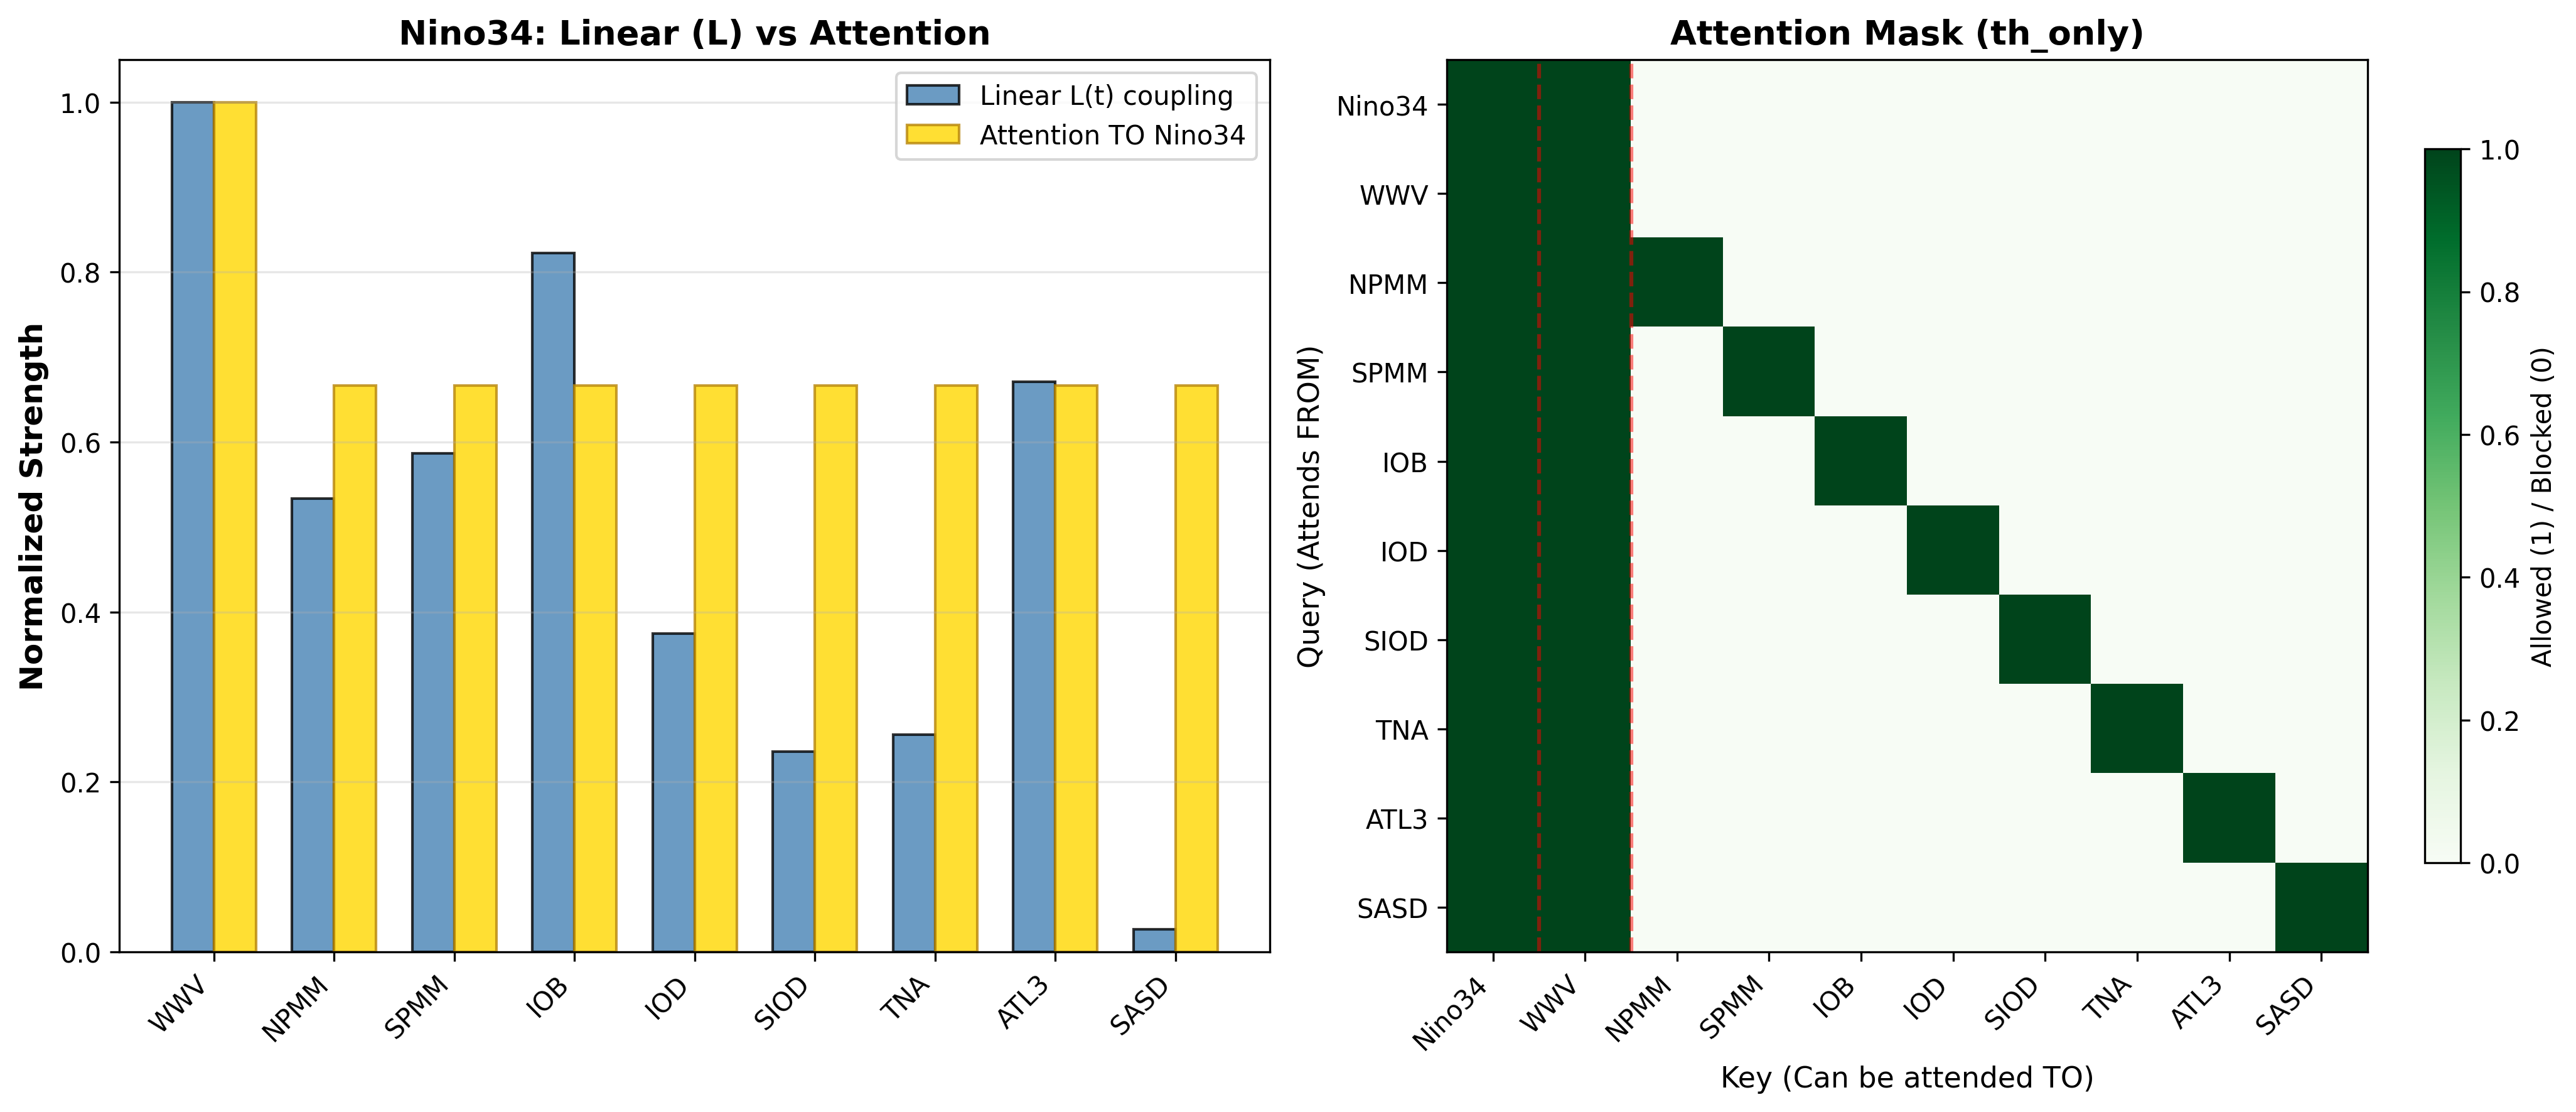
\includegraphics[width=\linewidth]{figures/linear_vs_attention.png}
%     \caption{The contribution from the linear and non-linear part of the NXRO-attention model.}
%     \label{fig:attn_linear_vs_nonlinear}
% \end{figure}

